\documentclass[12pt, letterpaper]{article} 

\usepackage{amsmath, amssymb, amsthm, enumerate, graphicx}

\title{MATH  HW }
\author{Dani Nguyen}
\date{Winter 2025}

\begin{document}
\maketitle
\graphicspath{ {./} }

\noindent \textbf{Question 1} 
\begin{verbatim}
import numpy as np
import matplotlib.pyplot as plt
import matplotlib.patches as patches
# add plot of unit circle
    fig, ax = plt.subplots(figsize=(6, 6))
    circle = patches.Circle((0, 0), 1, edgecolor='green', 
    facecolor='none', linewidth=2)
    ax.add_patch(circle)
    ax.set_xlim(-1, 1)
    ax.set_ylim(-1, 1)
# generate random points and plot them
    rng = np.random.default_rng(714)
    N = 100
    x = rng.uniform(-1, 1, N)
    y = rng.uniform(-1, 1, N)
    inside_circle = x**2 + y**2 <= 1
    ax.scatter(x[inside_circle], y[inside_circle], color='yellow', s=1)
    ax.scatter(x[~inside_circle], y[~inside_circle], color='blue', s=1)
# estimate pi
    tau = inside_circle.sum()
    pi_est = 4 * tau / N
# error term
    error = abs(np.pi - pi_est)
    (pi_est, error)
\end{verbatim}

\newpage
\begin{center}
\begin{tabular}{ c|c|c }
    N & $\pi_N$ & $e_N$ \\
    \hline
    100 & 3.28 & 0.1384\\
    1,000 & 3.052 & 0.0895\\
    10,000 & 3.118 & 0.0235\\
    100,000 & 3.13876 & 0.0028\\
\end{tabular}
\end{center}

\includegraphics{plotn100.png}
\newpage
\noindent \textbf{Question 2} \\
a. First we compute the CDF from the given PDF.
\begin{align*}
    F(x) &= 
    \begin{cases}
        0 & \text{if } x < 0\\
        \int_{0}^{1}xdx & \text{if } 0\le x \le 1\\
        \int_{0}^{1}xdx + \int_{1}^{2}(2-x)dx & \text{if } 1 < x \le 2\\
        1 & \text{if } x > 2
    \end{cases} \\
    &= 
    \begin{cases}
        0 & \text{if } x < 0\\
        \frac 12 x^2 & \text{if } 0\le x \le 1\\
        -1 + 2x - \frac 12 x^2 & \text{if } 1 < x \le 2 \\
        1 & \text{if } x > 2
    \end{cases}
\end{align*}
Now solve $F(x) = u$
\begin{align*}
    X = \begin{cases}
        \sqrt{2u} & \text{if } 0\le u \le \frac 12\\
        2 - \sqrt{2-2u} & \text{if } \frac 12 < x \le 1
    \end{cases}
\end{align*}

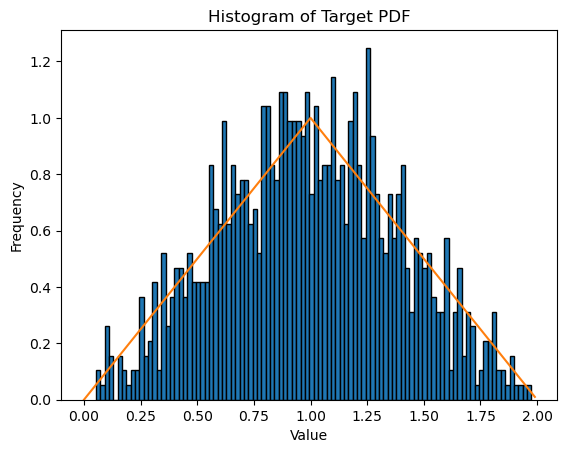
\includegraphics[scale=0.89]{histplot.png}

\noindent b. 





\noindent \textbf{Question 3} 

\end{document}